\section{Problem Statement}

% real-time
Even with the computing nodes closer, actors depending on real-time still can
not rely on unpredictable networks. It is however possible to get closer to
real-time computation by using edge-computing and new technologies. Current
research is mostly focusing on enhancing the network component using novel 5G
technologies~\cite{nunna_enabling_2015} and finding and evaluating new
protocols~\cite{suriyachai_survey_2012}, but research on improving response-time
on the edge node itself is scarce. There still however is potential on the edge
devices in the context of IIoT specifically. Frequently recurring requests, with
responses only depending on internal states or infrequently changing variables
currently require redundant overhead, such as context switches, which not only
costs valuable computing power on the edge node, but also unnecessarily delays
response.

In this thesis we'll consider the following scenario as visualized in
Figure~\ref{fig:communication_before}. An IIoT network consisting of many IoT
devices connected to an edge server which processes their requests. Most of
these request only require a simple reply based on an internal state, saved on
the edge server, which, compared to the incoming messages, only rarely changes.
This means that the server is constantly replying with the same message
containing that state. Now every single request has to go through the pipeline
and experiences a context switch to then be processed in the user space in the
Linux environment. This means it is scheduled with a low priority, possibly
delaying it even further. It is however necessary for these messages to be
processed as quickly as possible as that means that existing IoT devices can
fulfill their service quicker and safer and potentially that even more IoT
devices can be added to the network also increasing productivity.

\begin{figure}[htpb]
       \centering
       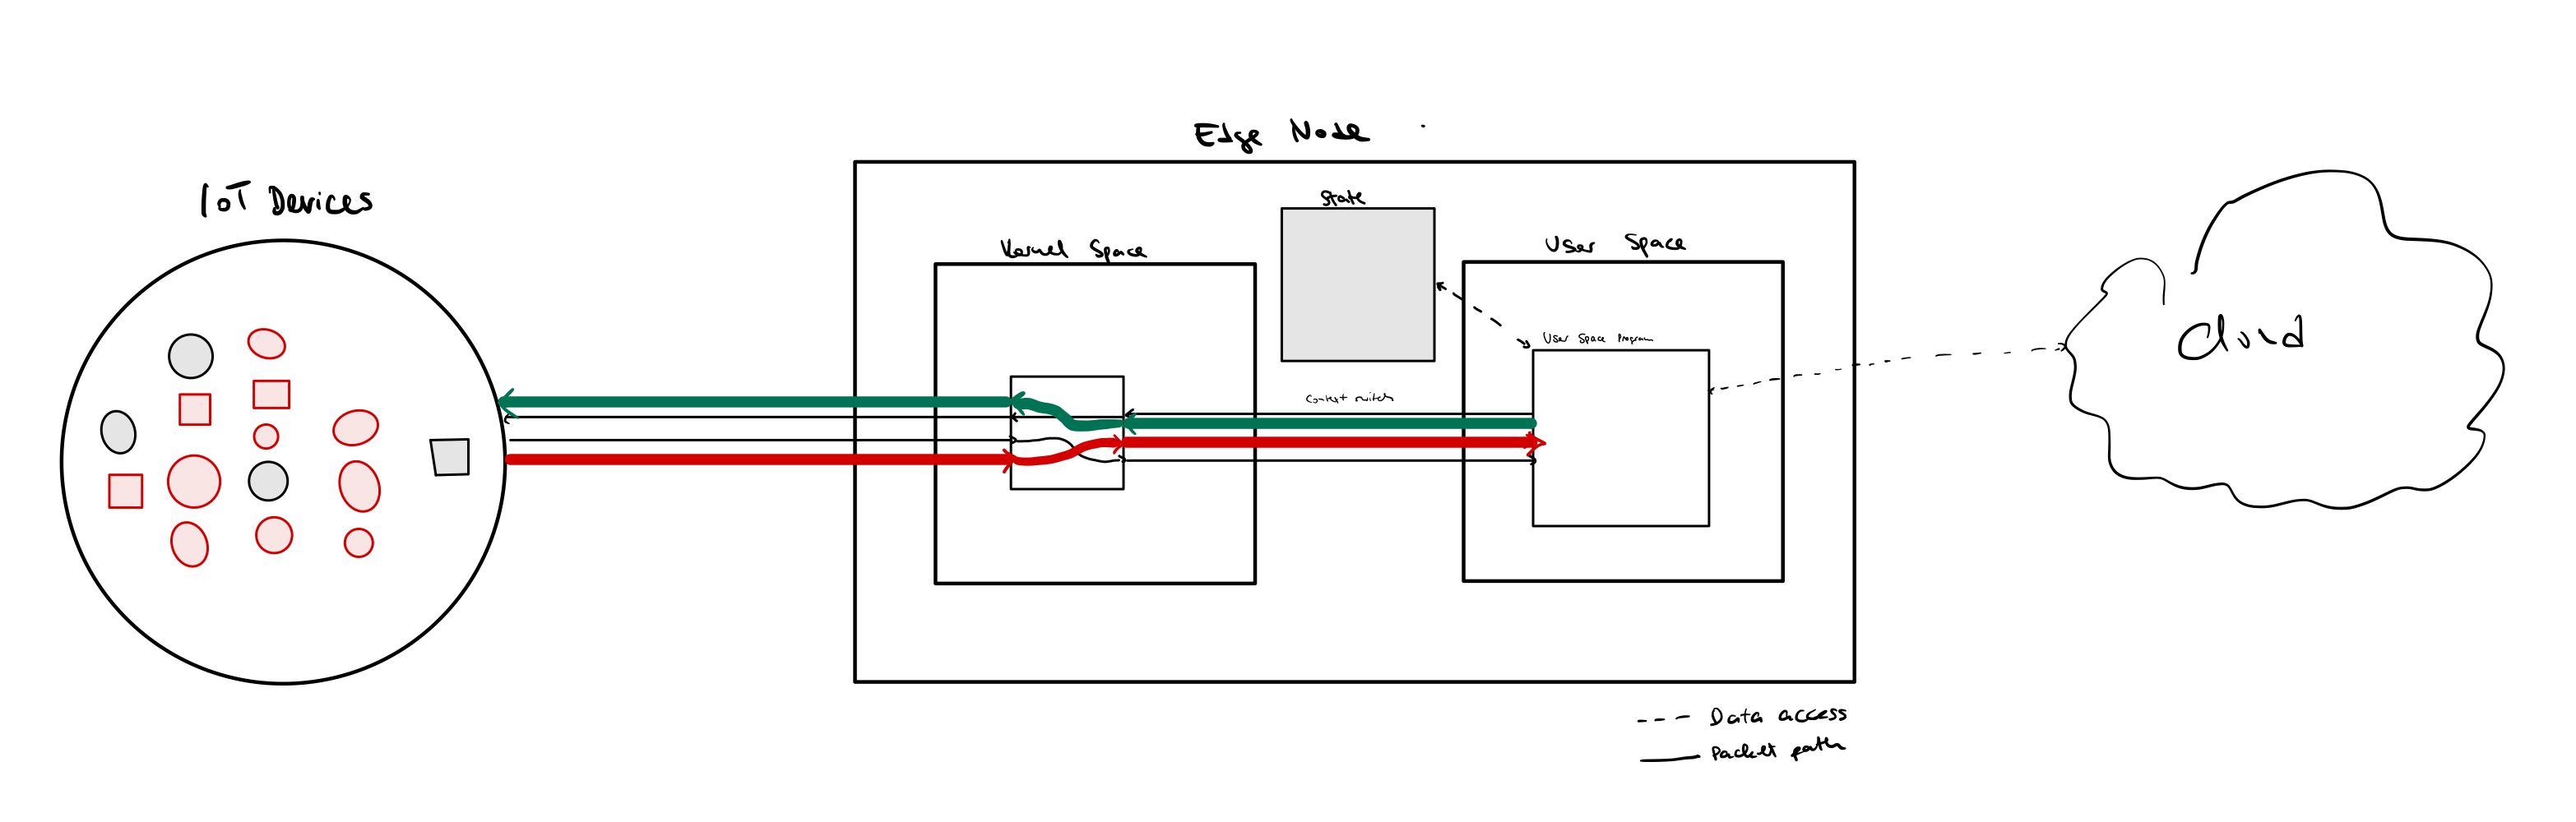
\includegraphics[width=\linewidth]{communication_before}
       \caption{communication before%
       \label{fig:communication_before}}%
\end{figure}
